% article example for classicthesis.sty
\documentclass[10pt,a4paper]{article} % KOMA-Script article scrartcl
\usepackage{import}
\usepackage{xifthen}
\usepackage{pdfpages}
\usepackage{transparent}
\newcommand{\incfig}[1]{%
    \def\svgwidth{\columnwidth}
    \import{./figures/}{#1.pdf_tex}
}
\usepackage{lipsum}     %lorem ipsum text
\usepackage{titlesec}   %Section settings
\usepackage{titling}    %Title settings
\usepackage[margin=10em]{geometry}  %Adjusting margins
\usepackage{setspace}
\usepackage{listings}
\usepackage{amsmath}    %Display equations options
\usepackage{amssymb}    %More symbols
\usepackage{xcolor}     %Color settings
\usepackage{pagecolor}
\usepackage{mdframed}
\usepackage[utf8]{inputenc}
\usepackage{longtable}
\usepackage{multicol}
\usepackage{graphicx}
\graphicspath{ {./Images/} }
\setlength{\columnsep}{1cm}

% ====| color de la pagina y del fondo |==== %
\pagecolor{white}
\color{black}



\begin{document}
    %========================{TITLE}====================%
    \title{{  7th Lab - Windows malware  }}
    \author{{Rodrigo Castillo and Juan Esteban Murcia}}
    \date{\today}

    \maketitle


    %=======================NOTES GOES HERE===================%
    \section{Theorical Lab}

        \subsection{Read the introduction to the Section "Analyzing Malicious Windows
            Programs" and explain why is it important to know the details of Windows OS
            (Windows API, user/kernel mode, execution of code outside a file)?}

            As a computer science student, is important to know details about
            Windows OS because is the most used operating system , as a forensics
            investigator, is important because most of the malware works for
            windows, somethimes, malware will use those libraries and services
            making the aknowledgment of those libraries really important for
            understanding and studyng malware and how it works.

        \subsection{Read the section "The Windows API" and identify which are the
            Windows API Types}.

            types of windows api:
            \begin{itemize}
                \item {WORD:}
                    is a unsigned 16bit value .
                \item {DWORD:}
                    is a unsigned 32bit value .
                \item {HANDLES:}
                    is a reference to an object , is not documented so it should
                    only be managed by windows APIs.
                \item {Long Pointer}
                    is a pointer to another type of variable.
                \item {Callback}
                    represents a function that is going to be called by a windows
                    API.
            \end{itemize}

        \subsection{Read the section "File System Functions" and explain the
        difference between shared files and files accesible via namespaces}

        shared files are special files which paths looks like  \textbf{$
        //nameserver/share  $}
        \textbf{or}   \textit{\textbf{\textbf{\textbf{$ //?/nameserver/share
        $}}}}. the symbol  tells the operating
        system to  not parse the string, in order to access longer
        filenames.
        Files accesible via namespaces:
        namespaces can be understood as the number of a folder, each one store
        different type of objects.
        lowest namespace is called \textbf{NT}  and it has access to all devices
        and  all namespaces exist inside \textbf{NT}.
        An example of files found within the NT namespace can be seen in the
        following figure:

        \begin{figure}[h]
            \centering
            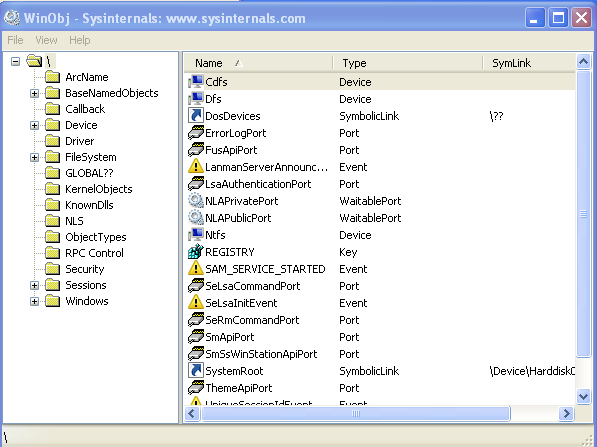
\includegraphics[scale=0.5]{1.png}
            \label{1}
            \caption{Namespace NT}
        \end{figure}

        \subsection{Read the section "The Windows Registry" and identify the place
        where executables (.exe) that start up when user log in may be configured.}
        A program that needs to start when a user logs in can be configured using
        the Run subkey using the Autoruns tool, that is a  free tool from Microsoft
        that list code and executables that will be executed on start up. In the
        following figure we can see the default programs that starts when the user
        logs in, and we can validate it is located in the Run subkey.

        \begin{figure}[h]
            \centering
            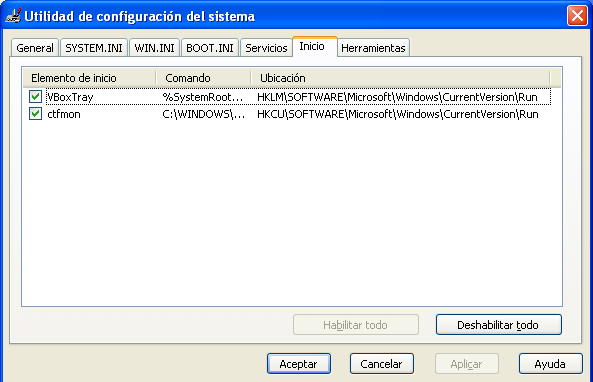
\includegraphics[scale=0.5]{2.png}
            \label{2}
            \caption{Startup programs}
        \end{figure}

        And here a screenshot of the Run subkey location using regedit:\newpage

        \begin{figure}[h]
            \centering
            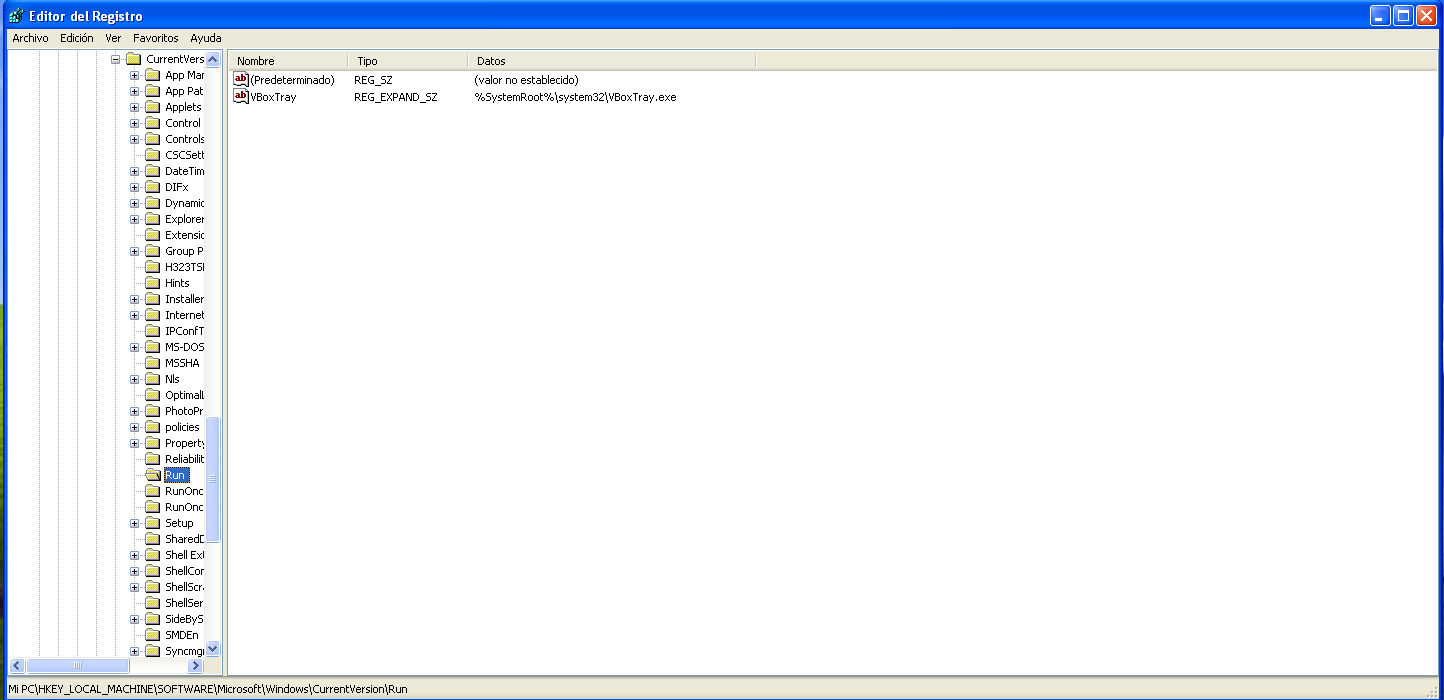
\includegraphics[scale=0.4]{3.png}
            \label{3}
            \caption{Run location}
        \end{figure}

        \subsection{Read the section "Common Registry Functions" and explain the
        difference between RegOpenKeyEx, RegSetValueEx and RegGetValue}

        \begin{itemize}
            \item RegOpenKeyEx\\
            Opens a registry for editing a query it contains a functions that
            allows to edit the registry without open it. Most of the programs use
            this one.
            \item RegSetValueEx\\
            It adds a value to a registry and modifies the data
            \item RegGetValue\\
            It returns the data found inside a registry.
        \end{itemize}

        \section{Explain the following assembly code. What is the purpose?}

        In the first place it calls the function RegOpenKeyEx to open the Run
        subkey, then it start handling and processing what we identified as a
        string to finally putting it in the Run registry using the function
        RegSetValueEx.

        \subsection{ Read the Section "The WinINet API" (Pag 178) and describe what
        the function InternetOpen does?}

        The WinInet API is a high level API which functions are stored in
        wininit.dll, if a  program imports functions from this library, it's using
        high level functions with networking purposes. One of those functions is
        InternetOpen that initialize an internet conection. But there are also
        other functions such as InternetOpenURL and InternetReadFile.

        \subsection{Read the section "Services" (Pag 185) and explain which are the
        main functions to manage services?}

        Another way to execute aditional code is stalling a \textit{service},
        because windows allows to run tasks using services. To achive this we have
        the three following functions:

        \begin{itemize}
            \item OpenSCManager, it returns a handle to the service, all code that
                wants to use a service approach must call this function.
            \item CreateService, This function adds a new service to the service
                control man ager, this allows the caller to specify where it will
                be executed and when it's going to be called.
            \item StartService, It starts a new service, it is only used if such
                service is going to be configured manually.
        \end{itemize}

        \subsection{Read the section "Interprocess Coordination with Mutexes" (Pag
        184), understand the following code and explain why is important a mutex?}

        Mutex refers to global objects, that coordinates several proceses and
        execution threads, generally they are used to control access to shared
        resources, but they are also used in malware, because if two different
        threads needs to access the same space, a mutex can control this
        operations. The assembly code what is basically doing is trying to open a
        mutex using the three arguments pushed to the stack, we assume that if the
        operation was successfull, it jumps to another part of the execution, else
        it proceed to create a the mutex with those three arguments, we can
        interpret that as creating the execution of a malware if and oly if such
        malare is not already in execution.

        \subsection{What is a SYSTEMTIME structure?}

        The systemtime structure specifies date and time, using members like month,
        day, year, weekday, minute, second and millisecond, it is either in UTC or
        in local time.

        \subsection{What the SetWaitableTimer function does?}

        It activates a specified waitable timer, when the due time arrives, the
        timer is signaled and the thread of the timer calls an optional routine.

        \subsection{Read the section "Creating a Thread" (Pag 182), understand the
        following code and explain in detail how a thread is set?}

        CreateThread function creates a new thread of execution, so what we can see
        in the code is ho the malware is creating 2 different threads with several
        mlicious purposes, for example load libraries in parallel to avoid stoping
        the malware execution or to avoid exiting a while, etc.

        \newpage
    \section{Practical Lab}

        \subsection{Identify in the "Strings" tab, some functions that may
            indicate that the malware configure a service (OpenSCManager,
            CreateService, etc).}

            \begin{figure}[h!]
                \centering
                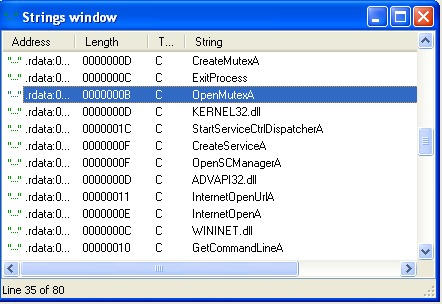
\includegraphics[width=0.8\linewidth]{4.png}
                \caption{Strings related to services}
                \label{stringsrelated}
            \end{figure}
            here, we can see that the functions that we identified previusly
            are in the source binary of the program, that mean that probably
            the program is consuming them. This make the previus section
            important to understand this kind of malware.

        \subsection{location of main}
            Using Ida we identified the location of main
            \begin{figure}[h!]
                \centering
                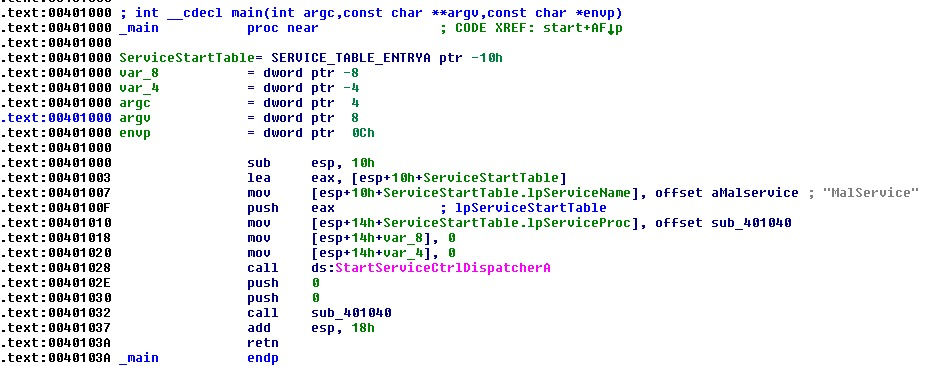
\includegraphics[width=0.8\linewidth]{loc.jpeg}
                \caption{location of main function}
                \label{locationmainfuction}
            \end{figure}
            main fuction is locaten at $ 0x00401000  $ .

            \newpage
        \subsection{Review the code inside function $ sub_401040  $  and observe that
            inside there is also a call to the funcion $ OpenMutexA.  $ }

            is calling a mutex function to check if malware is already created,
            if the malware is created, the  function call ends, but if is not
            created yet, the mutex for the malware is created.
            \begin{figure}[h!]
                \centering
                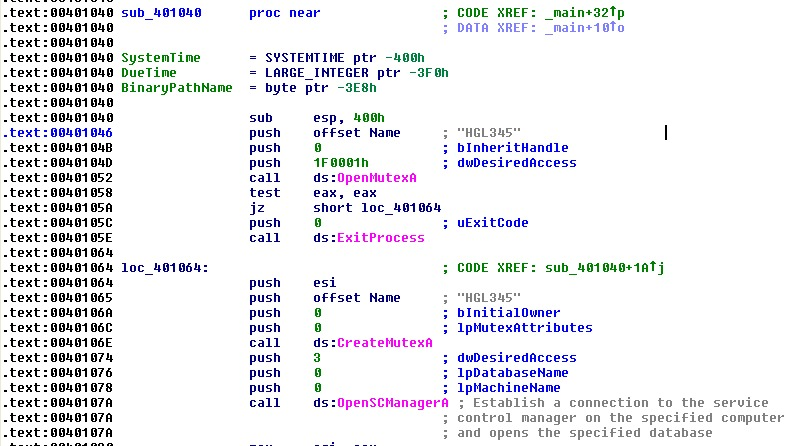
\includegraphics[width=1\linewidth]{mutef.jpeg}
                \caption{Mutex call}
                \label{mutex}
            \end{figure}

        \newpage
        \subsection{Analyze the code at the address 401064 and observe that at
            40106E there is a call to the function ds:CreateMutexA. Then, there
            is also a call to functions ds:OpenSCManager and
            ds:GetModuleFileName. ds:GetModuleFileName gets the full pathname
            to the running executable or Loaded DLL.}

            \begin{figure}[h!]
                \centering
                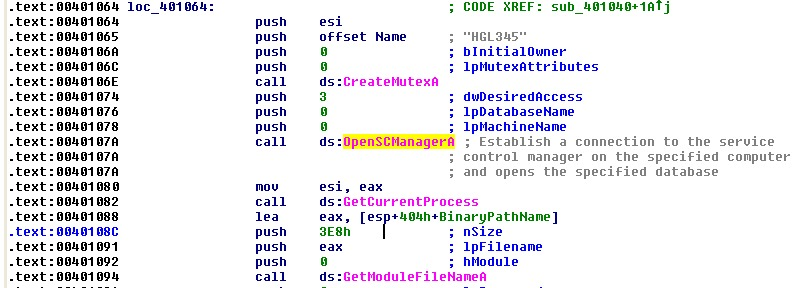
\includegraphics[width=0.5\linewidth]{lala.jpeg}
                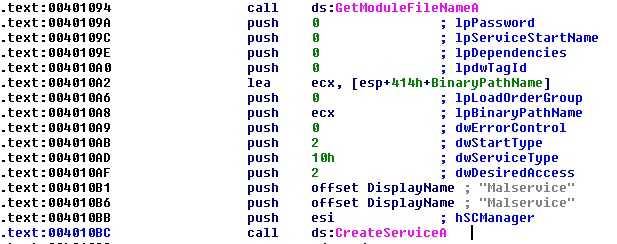
\includegraphics[width=0.5\linewidth]{serviciopath.jpeg}
                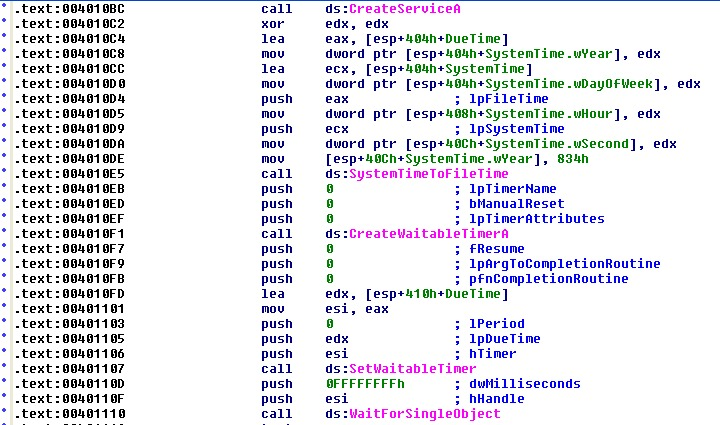
\includegraphics[width=0.5\linewidth]{jeje.jpeg}
                \caption{service path}
            \end{figure}

            \subsection{Observe that at address 004010C2 exitst a SYSTEMTIME...
            SystemTime.wYear is 834h. What does it mean}

            it means that is taking a variable in  system date,  and is
            modifying this date to year 2100.

    \section{Question:}
        \subsection{Q13: How does astaroth.exe ensure that it continues running
        (achieves persistence) when the computer is restarted?}

            creating itself as a service, as we know in previus section ,
            creating services will execute as autostart in windows when the
            sytem boots.

        \subsection{Q14: Why does astaroth.exe use a mutex?}
            creating itself as a service but only the first time or if the
            service was elimitated inorder to avoid creating the same service
            several times.

        \subsection{Q15: What is a good host-based signature to use for
        detecting astaroth.exe?}
            if there is a service that is wating untill year $ 2100  $  and it
            also importing mutex as a library is higly probable that this
            program is astaroth or similar malware. there are other several dll
            files that can be used to identify astaroth with more efficiency .

        \subsection{Q16: When will astaroth.exe finish executing?}
            in a day of the year $ 2100  $  .
















    %=======================NOTES ENDS HERE===================%1


    % bib stuff
    \nocite{*}
    \addtocontents{toc}{{}}
    \addcontentsline{toc}{section}{\refname}
    \bibliographystyle{plain}
    \bibliography{../Bibliography}
\end{document}
